% ==============================================================================
% PHẦN 2: THIẾT KẾ QUY TRÌNH, STORYBOARD, WIREFRAME VÀ PROTOTYPE
% ==============================================================================

% Slide 5: Quy trình As-Is vs To-Be
\begin{frame}{Đột phá trải nghiệm: Tái cấu trúc toàn diện 6 bước chăm sóc thú cưng}
  \footnotesize
  \begin{table}[H]
    \centering
    \begin{tabularx}{\textwidth}{p{1.8cm}X>{\bfseries\color{PetcarePrimary}}X}
      \toprule
      \textbf{Giai đoạn} & \textbf{Quy trình thủ công cũ (As-Is)} & Quy trình số hóa cải tiến (To-Be) \\
      \midrule
      1. Đặt lịch & Nhắn tin/gọi điện hỏi lịch, chờ phản hồi (15--45 phút). & Chọn trực tiếp trên ma trận khung giờ trống (30 giây). \\
      \addlinespace[1mm]
      2. Xác nhận & Xác nhận miệng/chat rời rạc, dễ trùng hoặc lỡ lịch. & Hệ thống cấp mã đặt lịch và xác nhận tức thì trên app. \\
      \addlinespace[1mm]
      3. Dặn dò dị ứng & Khai báo lại từ đầu, nhân viên dễ quên khi giao ca. & Hồ sơ y tế tự động đính kèm thẻ cảnh báo dị ứng. \\
      \addlinespace[1mm]
      4. Tiếp nhận & Nhắc miệng tại quầy tiếp tân, không có biên bản. & Quét mã QR Check-in, ký duyệt dặn dò y tế 2 lớp. \\
      \addlinespace[1mm]
      5. Theo dõi tiến độ & Mù mờ thông tin, lo lắng nhưng ngại gọi hỏi thăm. & Thanh tiến trình 4 mốc thời gian thực kèm Push Notification. \\
      \addlinespace[1mm]
      6. Lịch sử & Hóa đơn giấy dễ rách, thông tin da lông bị trôi mất. & Sổ nhật ký số hóa chi tiết loại dầu tắm \& xuất hóa đơn PDF. \\
      \bottomrule
    \end{tabularx}
  \end{table}
\end{frame}

% Slide 6: Storyboard
\begin{frame}{Hành trình trải nghiệm: Bảng phân cảnh 4 tình huống thực tế của Chị Lan}
  \begin{columns}[T]
    \begin{column}{0.62\textwidth}
      \centering
      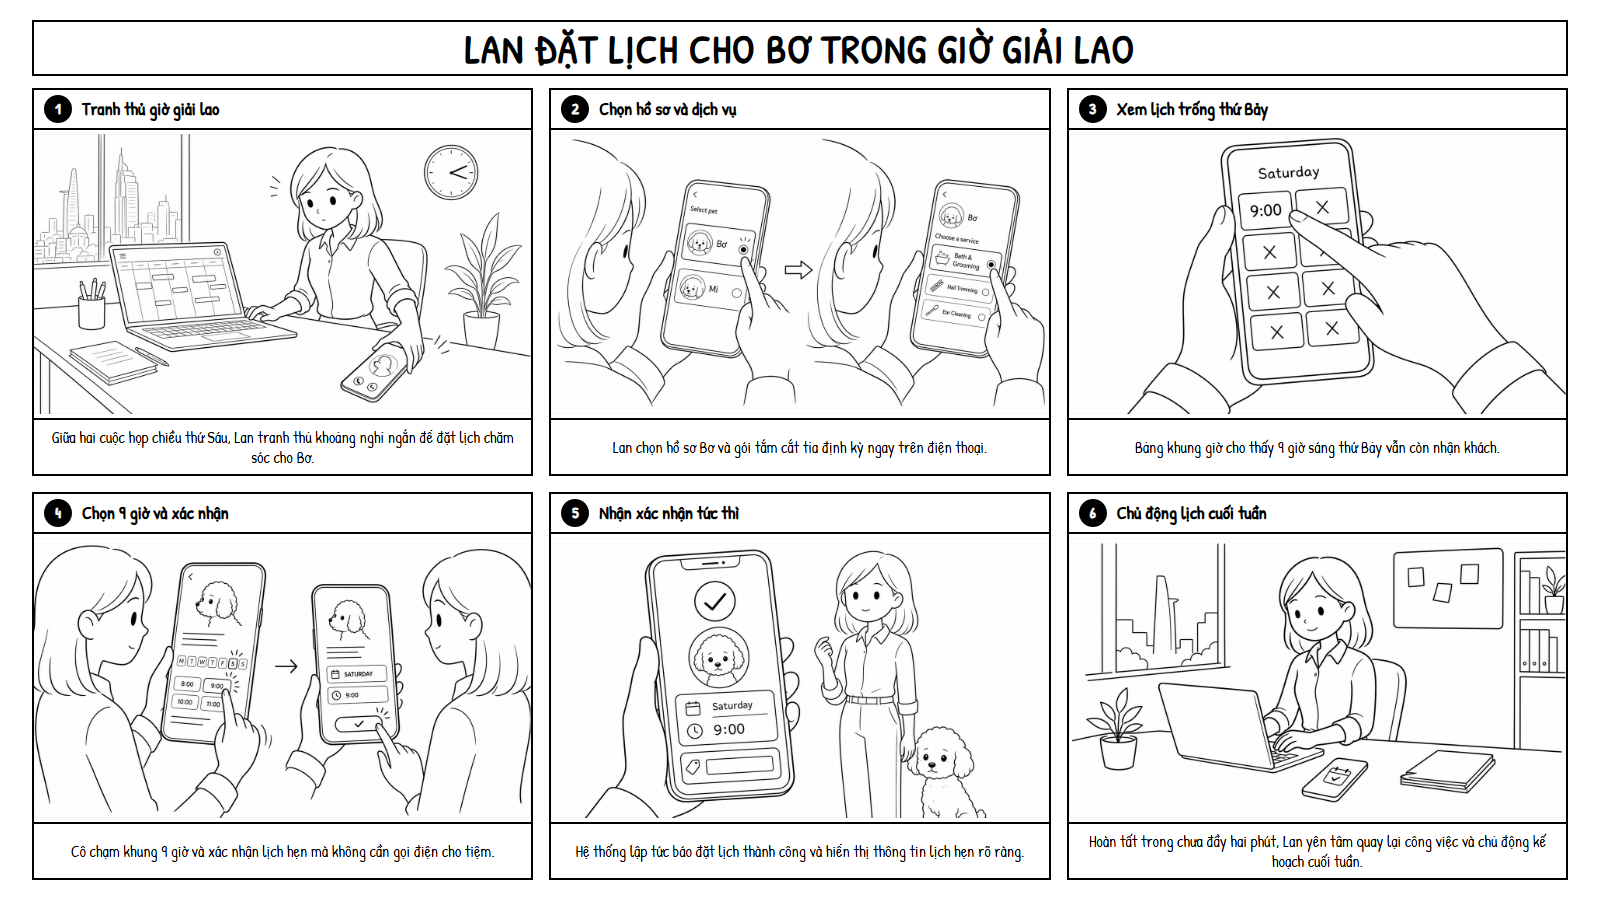
\includegraphics[width=\textwidth, height=0.72\textheight, keepaspectratio]{img/storyboard/storyboard-p1-g1.png}\\
      \vskip 1mm
      \footnotesize \textit{Minh họa Phân cảnh 1: Đặt lịch nhanh trong giờ giải lao tại văn phòng}
    \end{column}

    \begin{column}{0.36\textwidth}
      \begin{block}{4 Phân cảnh trải nghiệm}
        \footnotesize
        \begin{enumerate}
          \item \textbf{Tại văn phòng (T6):} Đặt lịch spa chiều thứ Bảy cho Bơ chỉ trong 30 giây giải lao.
          \item \textbf{Tại quầy tiếp nhận (T7):} Mã QR Check-in kích hoạt cảnh báo dị ứng xà phòng của Bơ.
          \item \textbf{Tại quán cà phê (T7):} An tâm làm việc qua 4 mốc tiến độ thời gian thực trên điện thoại.
          \item \textbf{Sau dịch vụ:} Xem lại tên dầu tắm dịu nhẹ và lưu phác đồ cho lần sau.
        \end{enumerate}
      \end{block}
    \end{column}
  \end{columns}
\end{frame}

% Slide 7: Wireframe & Kiến trúc thông tin
\begin{frame}{Kiến trúc thông tin \& Khung giao diện: Tối ưu chuẩn Mobile-first}
  \begin{columns}[T]
    \begin{column}{0.54\textwidth}
      \textbf{Kiến trúc thông tin 4 phân hệ cốt lõi:}
      \begin{itemize}
        \item \textbf{Trang chủ:} Thẻ lịch hẹn sắp tới \& lối tắt đặt lịch nhanh.
        \item \textbf{Đặt lịch:} Stepper từng bước, khóa tự động khung giờ kín.
        \item \textbf{Live Tracking:} 4 Mốc trực quan kèm bộ đếm ngược đón bé.
        \item \textbf{Hồ sơ \& Lịch sử:} Lưu thông tin y tế, mỹ phẩm và hóa đơn.
      \end{itemize}
      \vskip 2mm
      \begin{block}{Liên kết thiết kế tương tác trên Figma}
        \scriptsize \centering \vskip 1mm
        Trực tiếp trải nghiệm bộ khung giao diện:\\
        \vskip 1mm
        \href{https://www.figma.com/design/X92n63gTmwhhI20v7sRqzT/HCI?node-id=0-1&t=5QZaB3diSm5V1LRj-1}{\color{PetcareSecondary}\textbf{\underline{Mở Wireframe trên Figma}}}
        \vskip 1mm
      \end{block}
    \end{column}

    \begin{column}{0.22\textwidth}
      \centering
      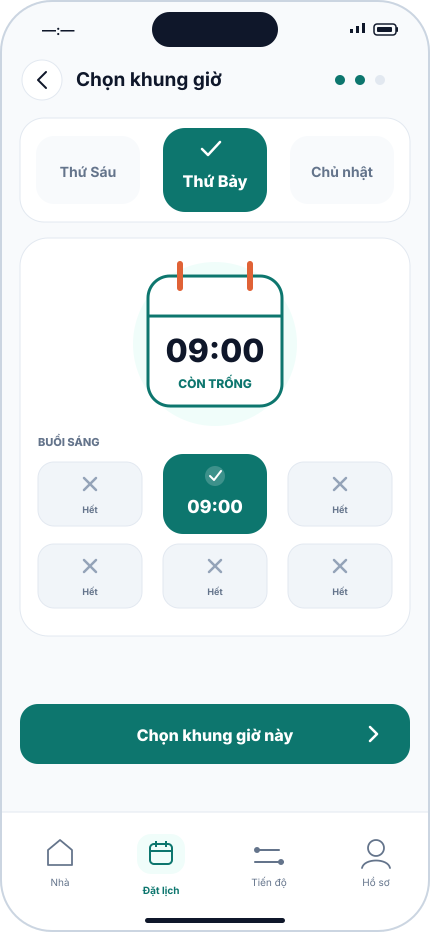
\includegraphics[width=\textwidth, height=0.70\textheight, keepaspectratio]{img/proto-p1/goal-1/03_choose_saturday_slot.png}\\
      \vskip 1mm
      \scriptsize (a) Ma trận chọn giờ
    \end{column}

    \begin{column}{0.22\textwidth}
      \centering
      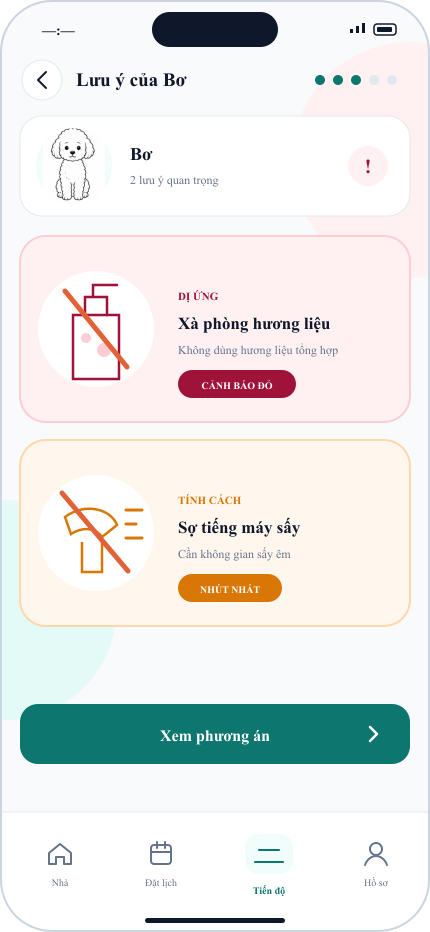
\includegraphics[width=\textwidth, height=0.70\textheight, keepaspectratio]{img/proto-p1/goal-2/03_profile_alerts.png}\\
      \vskip 1mm
      \scriptsize (b) Cảnh báo y tế
    \end{column}
  \end{columns}
\end{frame}

% Slide 8: Bản mẫu tương tác Figma
\begin{frame}{Bản mẫu tương tác Figma: 4 Trụ cột giải pháp cho Persona 1}
  \begin{columns}[T]
    \begin{column}{0.24\textwidth}
      \centering
      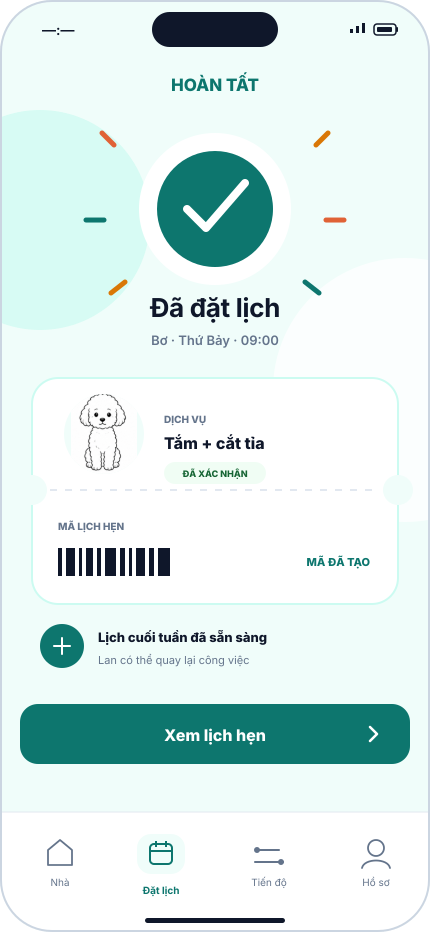
\includegraphics[width=\textwidth, height=0.64\textheight, keepaspectratio]{img/proto-p1/goal-1/05_booking_success.png}\\
      \vskip 1mm
      \scriptsize \textbf{1. Đặt lịch tức thì}\\
      \tiny Xác nhận lịch trong 30s
    \end{column}

    \begin{column}{0.24\textwidth}
      \centering
      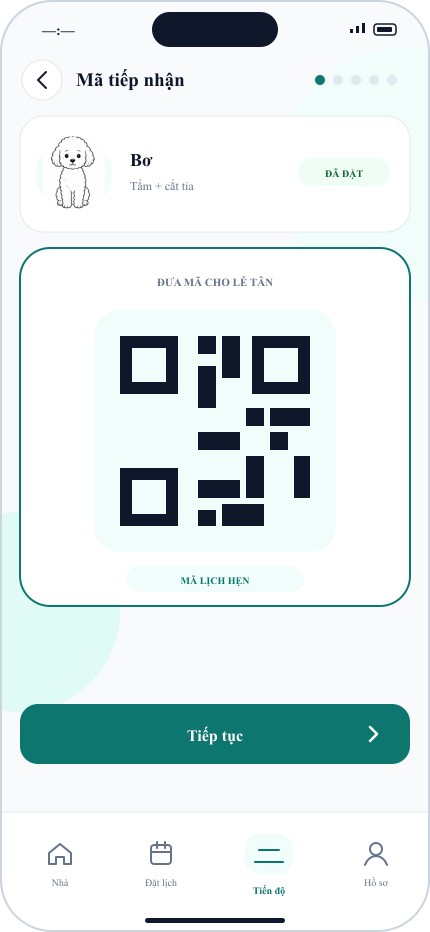
\includegraphics[width=\textwidth, height=0.64\textheight, keepaspectratio]{img/proto-p1/goal-2/01_show_checkin_code.png}\\
      \vskip 1mm
      \scriptsize \textbf{2. Tiếp nhận QR}\\
      \tiny Đồng bộ dặn dò dị ứng
    \end{column}

    \begin{column}{0.24\textwidth}
      \centering
      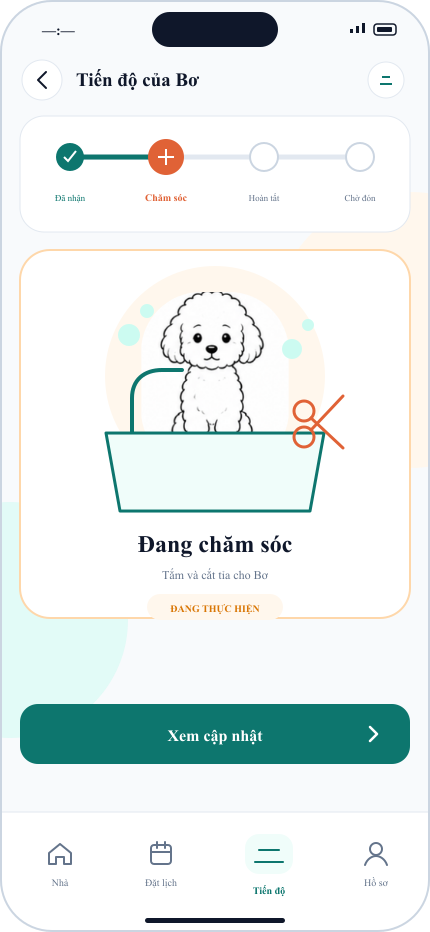
\includegraphics[width=\textwidth, height=0.64\textheight, keepaspectratio]{img/proto-p1/goal-3/02_step2_in_progress_care.png}\\
      \vskip 1mm
      \scriptsize \textbf{3. Live Tracking}\\
      \tiny 4 mốc thời gian thực
    \end{column}

    \begin{column}{0.24\textwidth}
      \centering
      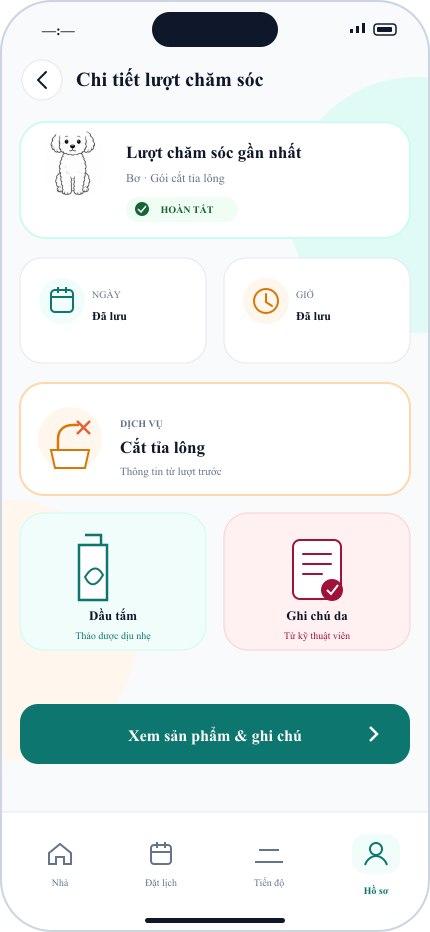
\includegraphics[width=\textwidth, height=0.64\textheight, keepaspectratio]{img/proto-p1/goal-4/03_session_details.png}\\
      \vskip 1mm
      \scriptsize \textbf{4. Lịch sử chi tiết}\\
      \tiny Nhật ký da lông \& chi phí
    \end{column}
  \end{columns}
  \vskip 3mm
  \centering
  \href{https://www.figma.com/design/X92n63gTmwhhI20v7sRqzT/HCI?node-id=0-1&t=5QZaB3diSm5V1LRj-1}{\normalsize\color{PetcareSecondary}\textbf{\underline{Trải nghiệm Prototype trực tiếp trên Figma (Nhấp vào đây)}}}
\end{frame}
